\chapter{Umsetzung}
\label{chap:umsetzung}

Die Umsetzung hatte drei Module als Ergebnis. Als erstes wurde eine wiederverwendbare Java Library entwickelt, welche genutzt werden kann, um Devices in das beschriebene Konzept zu integrieren. Der zweite Baustein ist eine Webapplikation, beschrieben im Abschnitt \ref{ums:devBrowser}, mit der die Device Descriptions interpretiert werden. Im Abschnitt \ref{ums:tinker} wird die Umsetzung eines Prototypen mit Tinkerforge Sensoren und Aktoren beschrieben.

\section{MQTT Device Description Library}
Um die Integration von Devices und das Erstellen von Device Description zu vereinfachen, wird eine Java Library entwickelt. Damit ist es möglich, Anwendungen für IoT Gateways in Java zu entwickeln.

Die Library übernimmt folgende Aufgaben:
\begin{itemize}
\item Handling der MQTT Verbindung zum Broker
\item Versenden von Event- und State Informationen mittels MQTT Messages
\item Empfangen von Command Messages
\item Einheitliche Abbildung der Devices und Topics
\item Hilfsklassen zur Erstellung der Device Descriptions
\end{itemize}

Die Parameter der Library (MQTT Broker URL, Application ID, etc.) können vom Anwender der Library konfiguriert werden.


\subsection{Klassendiagramm}

\begin{figure}[H]
	\centering
		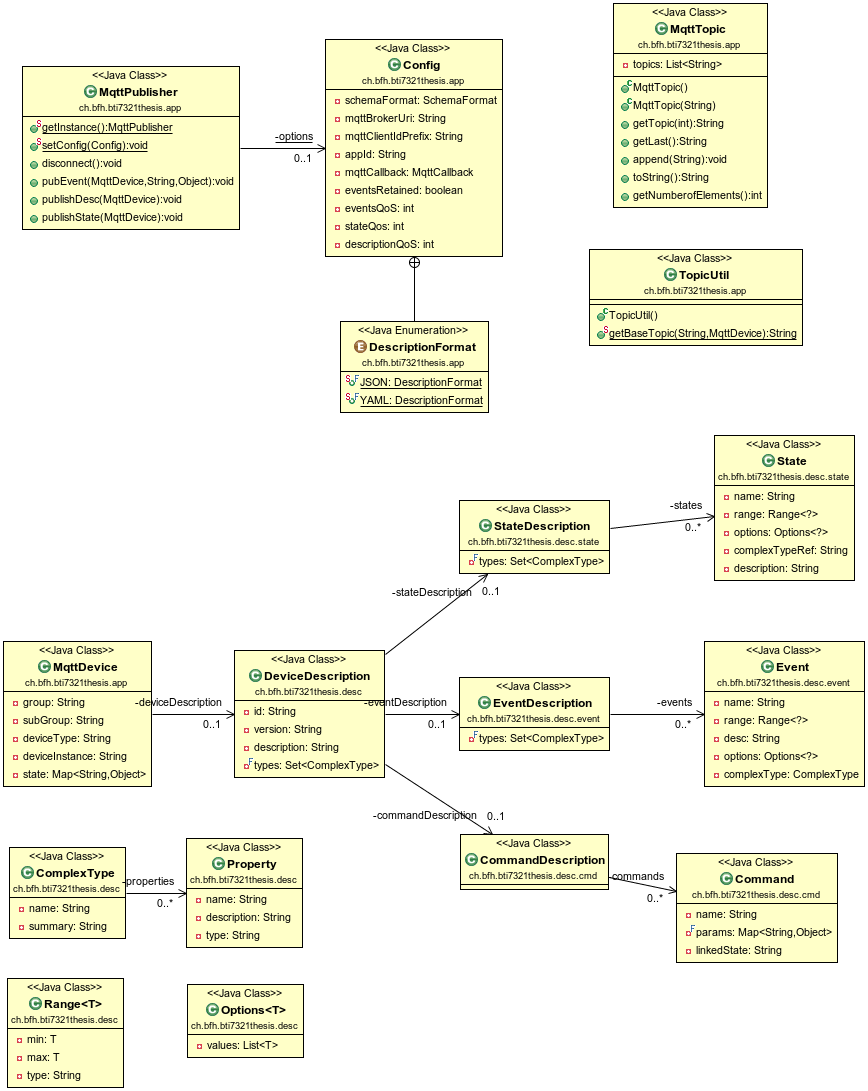
\includegraphics[width=1.0\textwidth]{diag/Lib_class_overview.png}
	\caption{Klassendiagramm MQTT Device Description Library}
\end{figure}

\begin{table}[H]
\begin{tabularx}{\textwidth}{|l|X|}

 \hline \rowcolor{lightgray}
 {\bf Klasse } & {\bf Zweck } \\  \hline
 
 MqttPublisher & Hauptklasse der Library. wird verwendet für das versenden der MQTT Nachrichten. \\ \hline

 Config & Wird verwendet, um bei der Initialisierung von MqttPublisher die Konfiguration abzugeben \\ \hline
 
 DescriptionFormat & Enum mit der Angaben zu den möglichen Formaten der Device Description.\\ \hline
 
 MqttTopic & Hilfsklasse die Abbildung von MQTT Topics.\\ \hline
 
 TopicUtil & Hilfsklasse für die Erstellung von MQTT Topics.\\ \hline
 
 MqttDevice & Klasse für die Abbildung von Devices. \\ \hline
 
 DeviceDescription & Enthält alle Attribute der Device Description.  \\ \hline
 
\end{tabularx}
\caption{Beschreibung der Klassen}
\end{table}

\subsection{Verwendung}
Die Device Description Library muss als erstes im eigenen Java Projekt eingebunden werden. Dies kann manuell mit der generierten .jar Datei (ch.bfh.barta3.mqttdevicedescription-1.0.0.jar) oder als Dependency Deklaration eines Maven Projektes getan werden.

\begin{listing}[H]
\begin{minted}[frame=single,
               framesep=3mm,
               linenos=false,
               xleftmargin=21pt,
               tabsize=4]{xml}
<dependency>
	<groupId>ch.bfh.barta3.mqttdevicedescription</groupId>
	<artifactId>ch.bfh.barta3.mqttdevicedescription</artifactId>
	<version>1.0.0</version>
</dependency>
\end{minted}
\caption{Maven Dependency MQTT Device Description Library}
\end{listing}

Als erstes muss die Konfiguration erstellt und an die Klasse \code{MqttPublisher} übergeben werden. Danach muss das Device inklusive Description erstellt werden. Sobald dies erfolgt ist, ist kann die Library beginnen, Daten zu versenden und reagiert auf empfangene Commands.

\begin{listing}[H]
\begin{minted}[frame=single,
               framesep=3mm,
               linenos=false,
               xleftmargin=21pt,
               tabsize=4]{java}

...

// Define Config
Config options = new Config();
options.setMqttBrokerUri("tcp://iot.eclipse.org:1883");
options.setAppId("myApp");
options.setMqttCallback(new MyCallbackHandler());
MqttPublisher.setConfig(options);
	
// Create Device and Description	
MqttDevice device = new MqttDevice("Bern", "Wankdorf", "Temp", "t1");	
device.setDeviceDescription(new DeviceDescription("test", "1.0"));
...

// Start publishing
MqttPublisher.getInstance().publishDesc(device);
MqttPublisher.getInstance().pubEvent(device, "event", "22");

...

\end{minted}
\caption{Einfaches Beipsiel für die Verwendung der Library}
\end{listing}

\textbf{Konfiguration} \\
Über das \code{Config} Objekt wird die Library konfiguriert. Für die als Pflichtfeld aufgeführten Parameter müssen Werte angegeben werden, ansonsten wird bei der ersten Verwendung eine entsprechende Exception ausgelöst. Die optionalen Parameter erhalten bei keiner Angabe des Anwenders den angegebenen Standardwert.


\begin{table}[H]
\begin{tabularx}{\textwidth}{|l|X|}

 \hline \rowcolor{lightgray}
 {\bf Parameter } & {\bf Beschreibung }  \\  \hline
 
 mqttBrokerUri & Pflichtfeld. URI des MQTT Brokers (inkl. Protokoll und Port) \newline Beispiel: tcp://iot.eclipse.org:1883 \\ \hline
 
 mqttClientIdPrefix & Präfix für die ClientIds der MQTT Connections. Es werden zwei Connections aufgebaut. Für das Publishing eine mit ClientId {[mqttClientIdPrefix]}\_pub und eine zweite Connection für das Empfangen von Messages mit ClientId {[mqttClientIdPrefix]}\_sub \newline Falls kein Wert angegeben wird, wird eine zufälliges Präfix generiert. \\ \hline
 
 appId & Pflichtfeld. Identifikation der Applikation. \\ \hline
 
 mqttCallback & Pflichtfeld. Implementation des Interfaces org.eclipse.paho.client.mqttv3.MqttCallback. Wird wird aufgerufen, wenn die Devices einen Command erhalten. \\ \hline
 eventsRetained &  true / false. Gibt an, ob die Event Messages mit Retained Flag versendet werden sollen. \newline Standard: true \\ \hline
 
 descriptionFormat & Format der Device Description. Mögliche Werte: YAML, JSON. \newline Standard: YAML \\ \hline
 
 eventsQoS & Gibt an, mit welcher \gls{qos} die Event Messages versendet werden sollen (0, 1, 2). \newline Standard: 1 \\ \hline
 
 stateQos & Gibt an, mit welcher \gls{qos} die State Messages versendet werden sollen (0, 1, 2). \newline Standard: 1 \\ \hline
 
 descriptionQoS & Gibt an, mit welcher \gls{qos} die Description Messages versendet werden sollen (0, 1, 2). \newline Standard: 1 \\ \hline
 
\end{tabularx}
\caption{Konfigurationsoptionen der Library}
\end{table}



\subsection{Verwendete Komponenten} {

Für die Umsetzung der MQTT Device Description Library wurden folgende Fremdkomponenten integriert:

\begin{table}[H]
\begin{tabularx}{\textwidth}{|l|X|}

 \hline \rowcolor{lightgray}
 {\bf Komponente } & {\bf Beschreibung }  \\  \hline
 
 Eclipse Paho & MQTT Client Implementation \newline \url{http://www.eclipse.org/paho} \\ \hline

 Jackson JSON Processor & JSON Serialisierung und Parsing \newline \url{http://wiki.fasterxml.com/JacksonHome} \\ \hline
 
 Jackson Modul YAML & Erweiterung der Jackson Library für das YAML Datenformat \newline \url{https://github.com/FasterXML/jackson-dataformat-yaml} \\ \hline
 
\end{tabularx}
\caption{Externe Komponenten}
\end{table}


\section{Device Browser} \label{ums:devBrowser}
Mit der entwickelten Webapplikation lassen sich die Device Descriptions übersichtlich darstellen. Die Applikation ist als reine Clientanwendung in Javascript umgesetzt.
Die Anwendung zeigt die auf einem Broker publizierten Devices in einer Liste an. Zu einem Device kann der Benutzer sich die Device Description im Klartext anzeigen lassen. Die Device Description wird interpretiert und unterteilt in die verschiedenen Bereiche werden die Attribute angezeigt.

\begin{figure}[H]
	\centering
		\frame{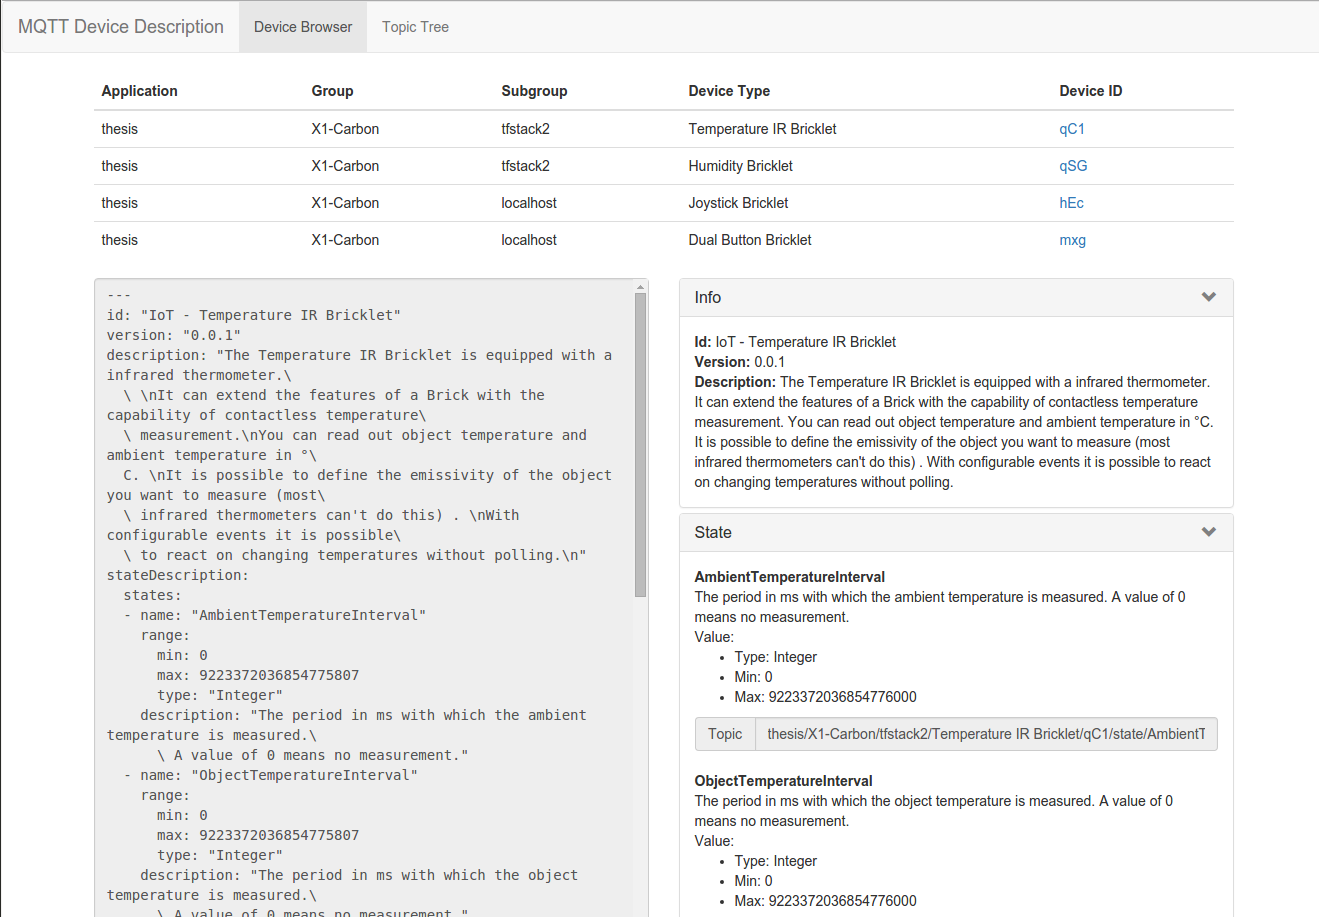
\includegraphics[width=1.0\textwidth]{bilder/device_browser_1.png}}
	\caption{Screenshot Device Browser}
\end{figure}


\newpage

\textbf{Bereich State} \\
Die State Objekte werden mit Beschreibung und den Typangaben angezeigt. Zudem wird das Topic ausgegeben, auf welchem die entsprechenden State Informationen publiziert wurden.


\textbf{Bereich Events}

\begin{figure}[H]
	\centering
        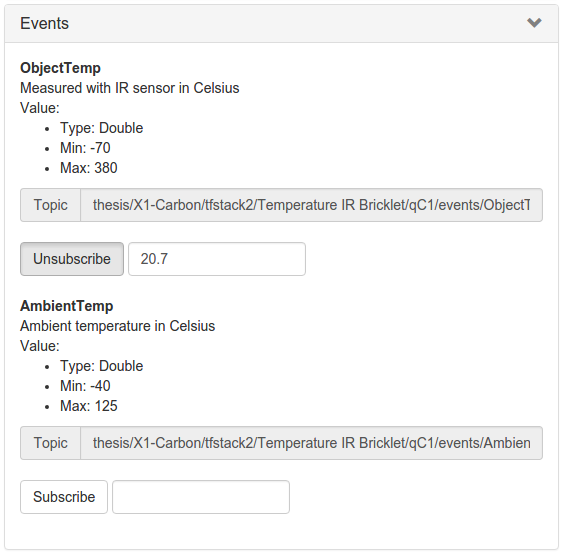
\includegraphics[width=0.7\linewidth]{bilder/device_browser_events.png} 
    \caption{Device Browser Event Darstellung}
\end{figure}

Die Event Informationen werden mit Name, Beschreibung und Angaben zum Typ angezeigt. Pro Event wird das Topic ausgegeben. Mit dem Betätigen der Schaltfläche 'Subscribe' verbindet sich die Webapplikation auf das Topic des Events und zeigt die empfangenen Daten im Textfeld an. Mit einem erneuten Klick auf die Schaltfläche wird die Verbindung beendet.

\newpage
\textbf{Bereich Commands}

\begin{figure}[H]
	\centering
        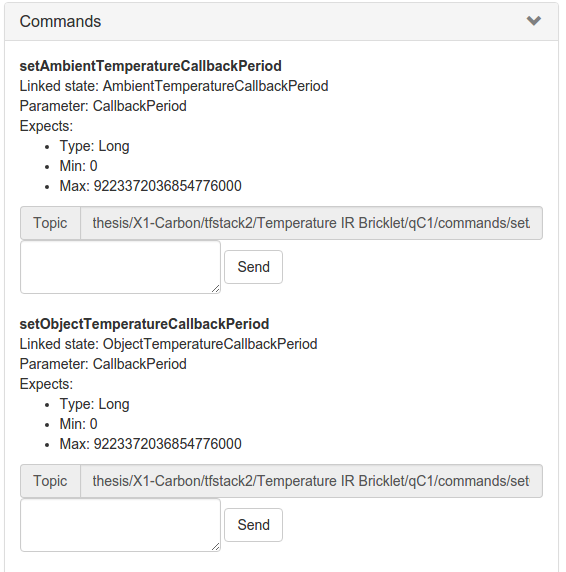
\includegraphics[width=0.7\linewidth]{bilder/device_browser_commands.png} 
    \caption{Device Browser Command Darstellung}
\end{figure}

Für die Command Objekte der Device Description werden nebst Name, Beschreibung und den erwarteten Typinforamtionen auch das Topic angezeigt, auf welches der Command gesendet werden muss. Es steht ein Eingabefeld zur Verfügung, in welchem der Payload der MQTT Message eingegeben werden kann. Mit dem Betätigen der Schaltfläche 'Send' wird der Command an das selektierte Device gesendet.


\textbf{Bereich Complex Types} \\
\begin{figure}[H]
	\centering
        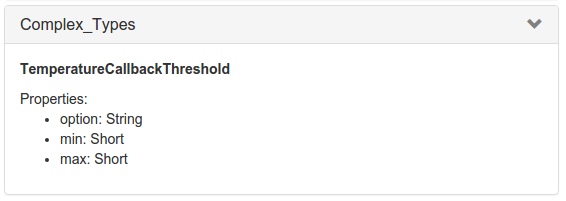
\includegraphics[width=0.7\linewidth]{bilder/device_browser_comptypes.png} 
    \caption{Device Browser Complex Type Darstellung}
\end{figure}

Falls das Schema Complex Types beinhaltet, werden diese hier aufgelistet. Für jeden Complex Type wird der Name und eine Liste der Properties (Attribute) aufgeführt.

\textbf{Topic Tree} \\
Als zweiter Teil der Webapplikation ist die Darstellung aller MQTT Topics des konfigurierten Brokers eingebunden. Dafür wurde die Applikation 'd3-MQTT-Topic-Tree' von Ben Hardill (\url{https://github.com/hardillb/d3-MQTT-Topic-Tree}) verwendet.

\begin{figure}[H]
	\centering
        \frame{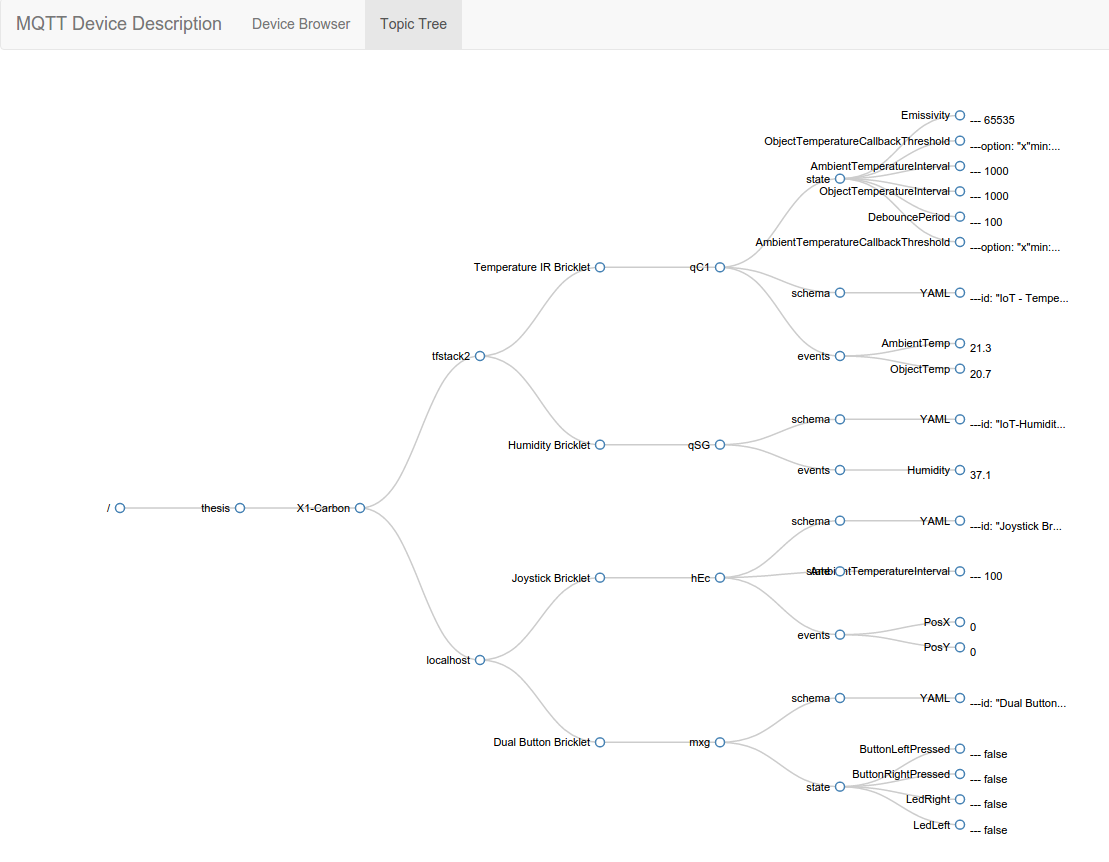
\includegraphics[width=1.0\linewidth]{bilder/topic_tree.png}}
    \caption{MQTT Topic Tree}
\end{figure}

Vor allen während der Entwicklung und dem Einbinden von neuen Devices hat sich diese Darstellung als sehr hilfreich erwiesen.

\subsection{Installation und Konfiguration}
Der MQTT Broker, auf den die Webapplikation zugreift, muss per Websockets erreichbar sein. Dafür eignet sich zum Beispiel der Mosquitto Broker. Während der Entwicklung der Applikationen wurde eine Mosquitto Installation mithilfe eines vorbereiteten Docker Images (\url{https://hub.docker.com/r/toke/mosquitto/}) durchgeführt und für sämtliche Tests verwendet.

Um die Webapplikation verwenden zu können, muss lediglich der Inhalt des Verzeichnisses \newline  \code{ch.bfh.bti7321thesis.schemabrowser} des Source Codes auf einen Webserver kopiert und die Datei \code{js/app/config.js} angepasst werden.

\begin{listing}[H]
\begin{minted}[frame=single,
               framesep=3mm,
               linenos=false,
               xleftmargin=21pt,
               tabsize=4]{js}

host = '46.101.165.125'; // hostname or IP address of broker
port = 9001;             // Websocket Port of broker
descFormat = 'YAML';     // YAML or JSON

\end{minted}
\caption{Beispiel Konfiguration Device Browser}
\end{listing}



%\newpage
\section{Anwendung Tinkerforge} \label{ums:tinker}

Um die MQTT Device Description Library an einem konkreten Beispiel zu testen, wurden verschiedene Bausteine des Tinkerforge Systems verwendet. Die Tinkerforge Bausteine (auch Bricklets genannt) haben den Vorteil, dass sie einfach zu verwenden sind und es bereits Libraries für die Kommunikation mit der Hardware gibt. Das Ziel der Anwendung war es zu demonstrieren, dass es möglich ist konkrete Devices mit dem entwickelten Konzept resp. der Device Description Library zu beschreiben und eine Interaktion von ausserhalb per MQTT zu ermöglichen.

\begin{figure}[H]
	\centering
        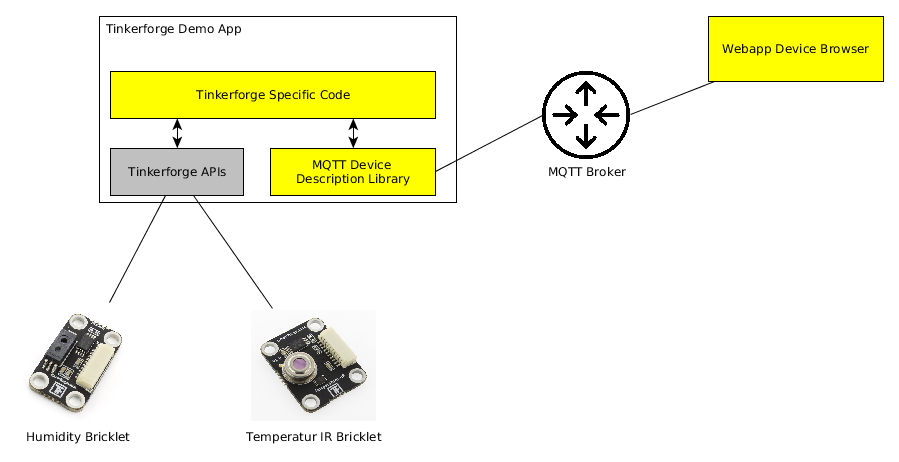
\includegraphics[width=1.0\linewidth]{diag/tf_arch.png}
    \caption{Aufbau der Tinkerforge Anwendung}
\end{figure}

\newpage
Folgende Sensoren resp. Aktoren wurden für die Integration ausgewählt:

\def\imagetop#1{\vtop{\null\hbox{#1}}}

\begin{table}[H]
\begin{tabularx}{\textwidth}{|l|X|l|}

 \hline \rowcolor{lightgray}
 {\bf Device } & {\bf Beschreibung } & \textbf{Bild} \\  \hline
 
 Sensor Luftfeuchtigkeit & Misst die relative Luftfeuchtigkeit. 
 \newline Mehr Informationen: \newline \url{http://www.tinkerforge.com/en/doc/Hardware/Bricklets/Humidity.html} & 
 \imagetop{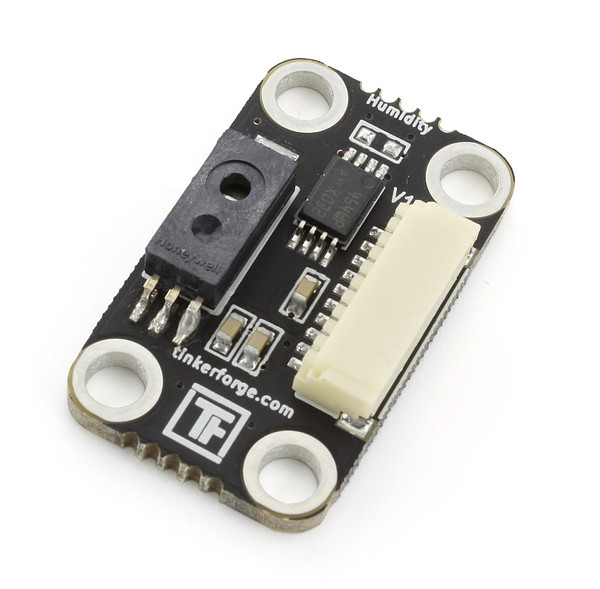
\includegraphics[width=0.4\linewidth]{bilder/bricklet_humidity.jpg}}    \\ \hline
 
 Sensor Temperatur Infrarot & Besteht einem Temperatursensor für die Umgebung und einem Infrarotsensor für die Messung der Objekttemperatur. \newline 
 \newline Mehr Informationen: \newline \url{http://www.tinkerforge.com/en/doc/Hardware/Bricklets/Temperature_IR.html} & 
 \imagetop{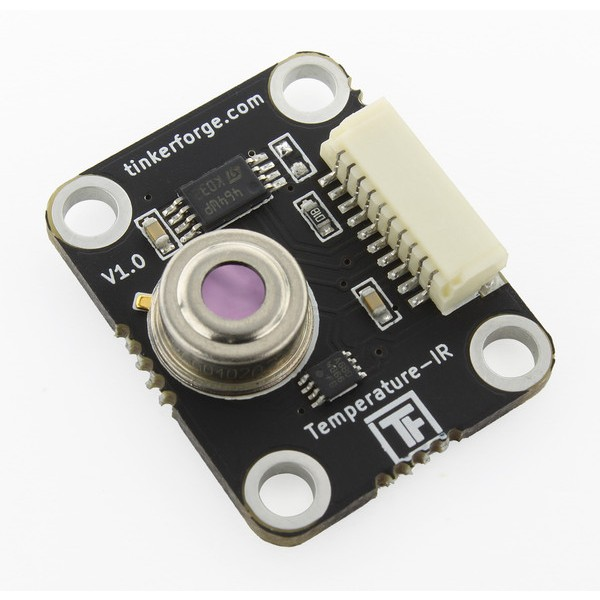
\includegraphics[width=0.4\linewidth]{bilder/bricklet_temperature_ir.jpg}}    \\ \hline
 
 Dual Button & Besteht aus zwei Buttons, welche je ein LED integriert haben. \newline 
 \newline Mehr Informationen: \newline \url{http://www.tinkerforge.com/en/doc/Hardware/Bricklets/Dual_Button.html} & 
 \imagetop{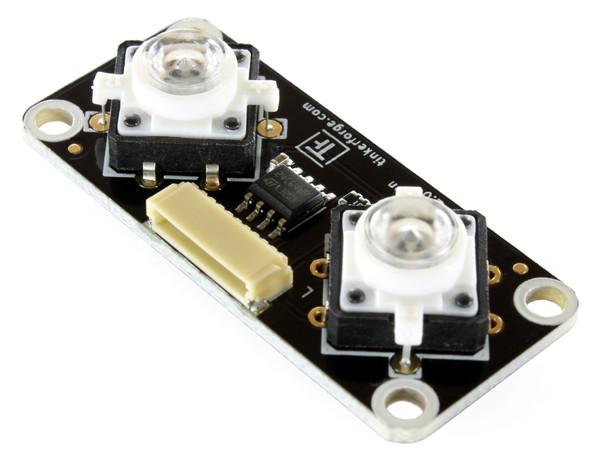
\includegraphics[width=0.4\linewidth]{bilder/bricklet_dual_button.jpg}}    \\ \hline

 \end{tabularx}
\caption{Verwendeten Tinkerforge Komponenten}
\end{table}

Quelle Bilder: \url{http://www.tinkerforge.com/en/doc/index.html}



\subsection{Klassendiagramm}

\begin{figure}[H]
	\centering
        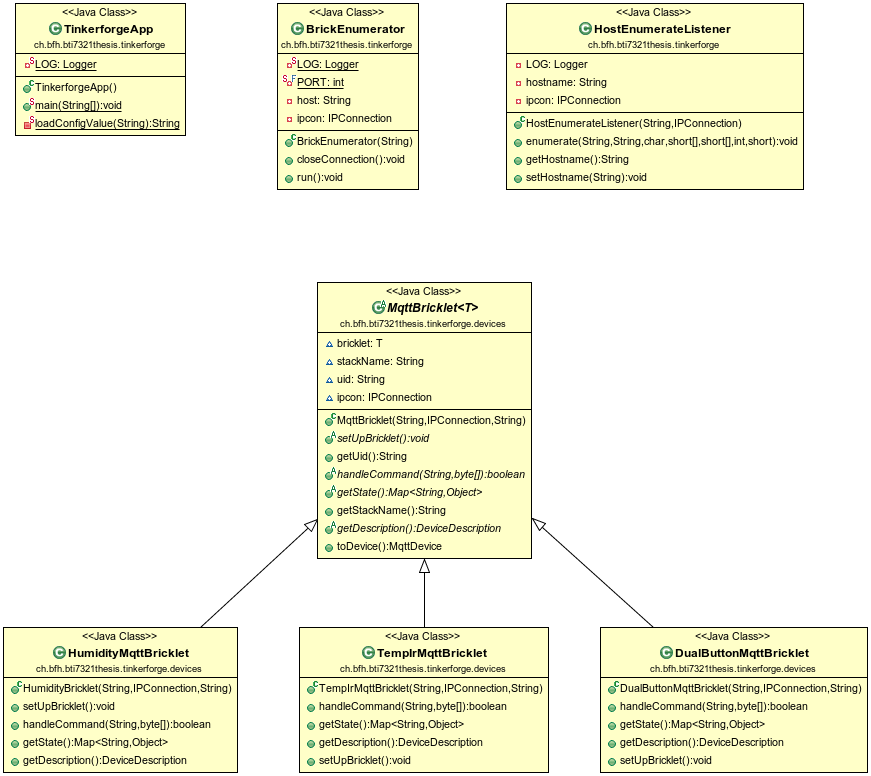
\includegraphics[width=1.0\linewidth]{diag/tf_overview_class.png}
    \caption{Klassendiagramm Tinkerforge Anwendung}
\end{figure}

\begin{table}[H]
\begin{tabularx}{\textwidth}{|l|X|}

 \hline \rowcolor{lightgray}
 {\bf Klasse } & {\bf Zweck } \\  \hline
 
 TinkerforgeApp & Start der Applikation, Einlesen der Konfiguration, Setup der MQTT Device Description Library. \\ \hline

 BrickEnumerator & Thread, welcher für jeden angegebenen Tinkerforge Stack die Devices (Bricklets) sucht. \\ \hline
 
 HostEnumerateListener & Empfängt die gefundenen Tinkerforge Devices und erstellt die entsprechenden \code{MqttBricklets} \\ \hline
 
 MqttBricklet &  Abstrakte Oberklasse für die konkreten Bricklet Implementationen. Definiert die abstrakten Methoden \code{setUpBricklet()}, \code{getState()}, \code{handleCommand(...)},  und \code{getDescription()}, welche von den Subklassen implementiert werden. \newline Mit der Methode \code{toDevice()} wird eine Instant der Klasse \code{MqttDevice} erzeugt, welche die Subklassen verwenden um z. Bsp. Events zu versenden. \\ \hline
 
 HumidityMqttBricklet &  Implementation für das Humidity Bricklet. \\ \hline
 
 TempIrMqttBricklet & Implementation für das Temperatur IR Bricklet. \\ \hline
 
 DualButtonMqttBricklet & Implementation für das Dual Button Bricklet.\\ \hline
 

\end{tabularx}
\caption{Beschreibung der wichtigsten Klassen}
\end{table}

\subsection{Device Descriptions}
Die Device Descriptions der drei behandelten Devices sind im Anhang \ref{app:device_descriptions} zu finden.

